\documentclass{beamer}

\usetheme{Warsaw}
\usecolortheme{seahorse}


\usepackage[french]{babel}
\usepackage[utf8]{inputenc}
\usepackage[T1]{fontenc}

\AtBeginSection[]
{
    \begin{frame}
        \frametitle{Table des matières}
        \tableofcontents[currentsection]
    \end{frame}
}


\begin{document}

\title{Algorithmes approchés}

\author{Arpad Rimmel}
\institute{SUPELEC}


\begin{frame}
    \titlepage
\end{frame}


\section{Introduction}


\begin{frame}
    \frametitle{Introduction}
    
    Catégories de problèmes étudiés:
    \begin{itemize}
        \item Problèmes ayant une complexité trop importante pour être résolue en un temps raisonnable.

        Exemple: exploration d'arbre avec un grand nombre de nœuds.

        \item Problèmes où il est impossible de trouver une solution optimale.

        Exemple: optimisation d'une fonction continue sans propriété.
    \end{itemize}

    Utilisation d'algorithmes donnant la meilleur solution possible en un temps donné.

\end{frame}


\section{Travaux précédents}

\begin{frame}
    \frametitle{Exploration d'arbre}
    Problème: prendre des décisions dans un environnement discret, observable, avec horizon fini et avec récompenses.
\\~
    \begin{columns}
    \begin{column}[l]{5cm}
        Exemple:
        \begin{itemize}
            \item multiplication de matrices
            \item jeu de Go
            \item samegame
            \item POMDP
            \item ...
        \end{itemize}
    \end{column}
    \begin{column}[r]{5cm}
        \begin{center}
            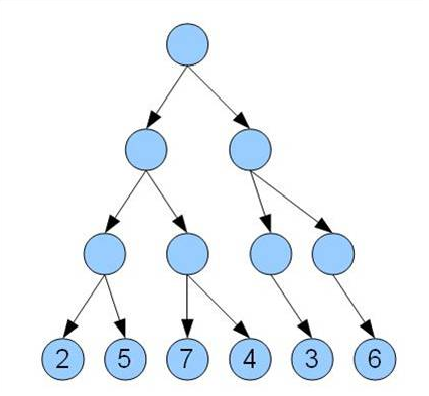
\includegraphics[scale=0.4]{tree.jpg}
        \end{center}
    \end{column}
    \end{columns}

\end{frame}

\begin{frame}
    \frametitle{Bandit Based Monte Carlo Tree Search}
    \begin{itemize}
        \item Basé sur la formule du bandit
        \item Évaluation par simulation Monte Carlo
        \item Performant pour les applications où la première décision est importante
    \end{itemize}
    \begin{center}
        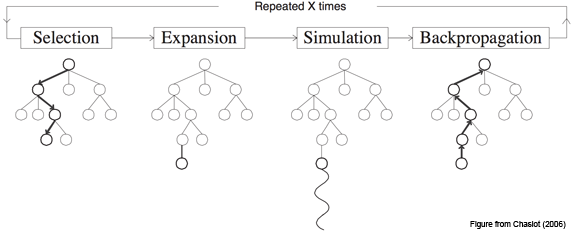
\includegraphics[scale=0.5]{mcts-algorithm.png}
    \end{center}

\end{frame}

\begin{frame}
    \frametitle{Nested Monte Carlo Tree Search}
    \begin{itemize}
        \item Basé sur une récursion d'évaluations
        \item Évaluation par simulation Monte Carlo
        \item Performant pour les applications où toutes les décisions sont importantes
    \end{itemize}
    \begin{center}
        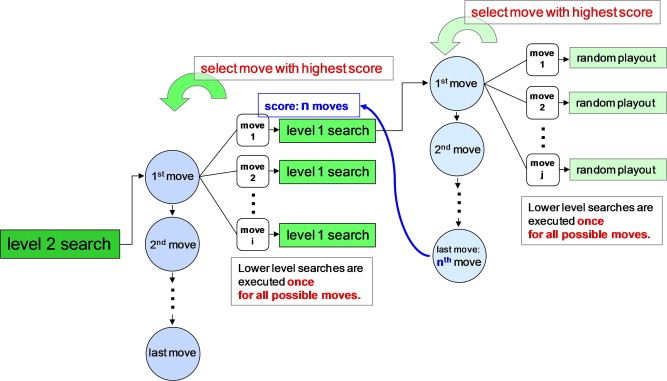
\includegraphics[scale=0.5]{nested-algorithm.jpg}
    \end{center}

\end{frame}


\begin{frame}
    \frametitle{Optimisation}
    Problème: 
    \begin{itemize}
    \item Trouver le maximum d'une fonction "boite noire".
    \item on peut obtenir la valeur en un point donné.
    \item Espace de recherche trop grand pour être exploré en entier.
    \end{itemize}

    \begin{center}
        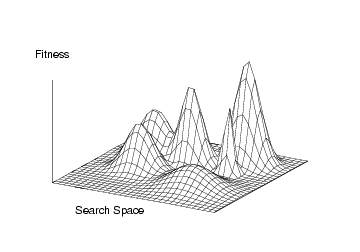
\includegraphics[scale=0.5]{multimodalFitnessLandscape.jpg}
    \end{center}

\end{frame}

\begin{frame}
    \frametitle{Algorithmes Evolutionnaires}

    \begin{itemize}
        \item Basé sur l'évolution d'une population d'individus
        \item Chaque individu correspond à un point 
        \item Le score de chaque individu correspond à la valeur de la fonction en ce point
        \item De nouveaux individus sont générés à partir des scores précédents
    \end{itemize}
    \begin{center}
        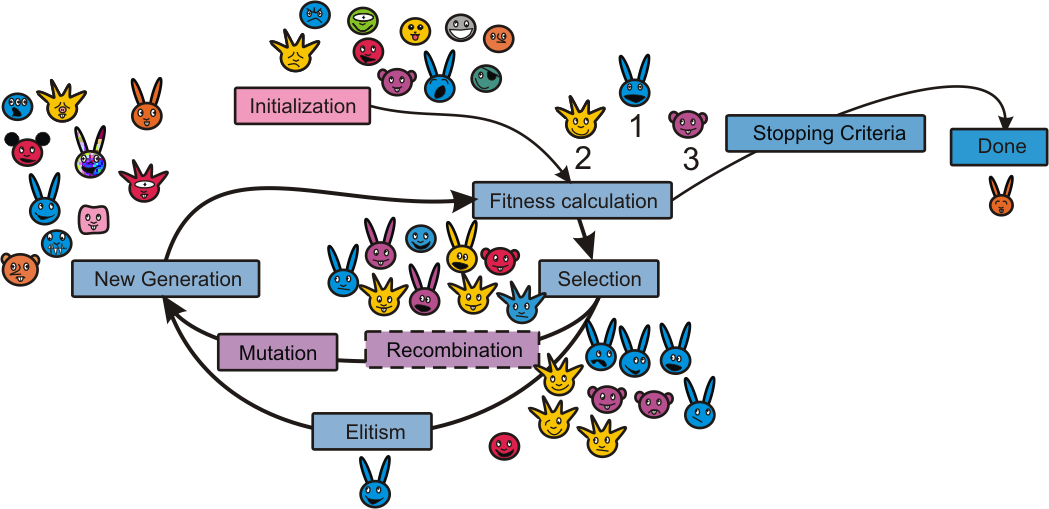
\includegraphics[scale=0.3]{EAalgorithmPedagogical.png}
    \end{center}


\end{frame}




\section{Travaux actuels}

\begin{frame}
    \frametitle{Carrés latins}
    But:
    \begin{itemize}
        \item Placer $n$ points dans une hypercube de taille $n$ par $n$.
        \item todo: pour une dimension donnée, chaque point doit avoir une valeur différente.
        \item todo: trouver la solution où la distance minimale entre 2 points est maximale.
    \end{itemize}
    Applications:
    \begin{itemize}
        \item Planification d'expériences
    \end{itemize}
    \begin{center}
        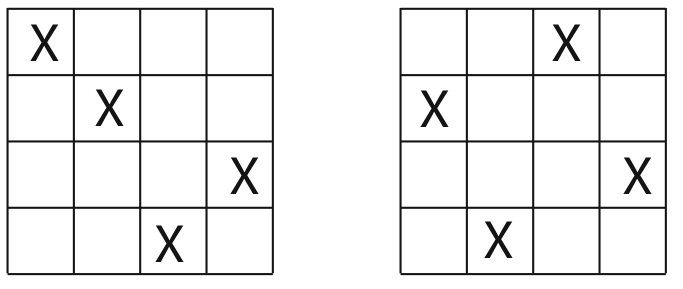
\includegraphics[scale=0.3]{LHS.jpg}
    \end{center}

\end{frame}

\begin{frame}
    \frametitle{Etat de l'art}
    \begin{itemize}
    \item En dimension 2, pour les normes $L_1$ et $L_{inf}$, des algorithmes donnant la solution optimale en un temps linéaire ont été fournis.
    \item Pour la norme $L_2$, uniquement des solutions approchées.
    \item En dimension supérieure à 2, uniquement des solutions approchées.
    \end{itemize}
\end{frame}

\begin{frame}
    \frametitle{Travaux préliminaires}
    Pour le moment 2 algorithmes testés:
    \begin{itemize}
        \item Nested Monte Carlo Tree Search

        Problème: pas vraiment une structure d'arbre.
        \item Algorithme génétique

        Résultat prometteurs.
    \end{itemize}
\end{frame}


\section{Perspectives}

\begin{frame}
    \frametitle{Perspectives}
    todo
    \begin{itemize}
        \item trouver des chemins dans des graphes
        \item trouver des colorations pondérées
    \end{itemize}
\end{frame}



\end{document}
